\documentclass[tikz]{standalone}
\usetikzlibrary{arrows,positioning}
\newcommand{\tikzsetnextfilename}[1]{}

\definecolor{pGray}{gray}{0.6}
\definecolor{pOrange}{RGB}{245,140,85}

\tikzset{
    circ/.style={circle, draw, inner sep=1pt, minimum width=1.3em, fill=pOrange},
    vert/.style={circle, draw, inner sep=1pt, minimum width=0.6em, fill=pOrange}
}

\begin{document}
\tikzsetnextfilename{6-vertex-model-1}
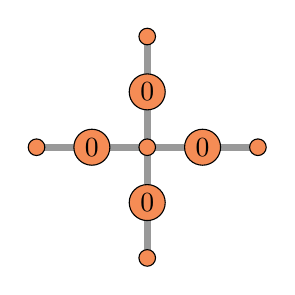
\begin{tikzpicture}[x=2em,y=2em,scale=1.0]
\draw[line width=2.5\pgflinewidth,pGray] (-2,0)--(2,0);
\draw[line width=2.5\pgflinewidth,pGray] (0,-2)--(0,2);
\node[circ] at (-1, 0) {$0$};
\node[circ] at ( 1, 0) {$0$};
\node[circ] at ( 0,-1) {$0$};
\node[circ] at ( 0, 1) {$0$};
\node[vert] at ( 0, 0) {};
\node[vert] at (-2, 0) {};
\node[vert] at ( 2, 0) {};
\node[vert] at ( 0,-2) {};
\node[vert] at ( 0, 2) {};
\end{tikzpicture}

\tikzsetnextfilename{6-vertex-model-2}
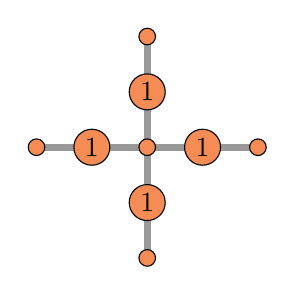
\begin{tikzpicture}[x=2em,y=2em,scale=1.0]
\draw[line width=2.5\pgflinewidth,pGray] (-2,0)--(2,0);
\draw[line width=2.5\pgflinewidth,pGray] (0,-2)--(0,2);
\node[circ] at (-1, 0) {$1$};
\node[circ] at ( 1, 0) {$1$};
\node[circ] at ( 0,-1) {$1$};
\node[circ] at ( 0, 1) {$1$};
\node[vert] at ( 0, 0) {};
\node[vert] at (-2, 0) {};
\node[vert] at ( 2, 0) {};
\node[vert] at ( 0,-2) {};
\node[vert] at ( 0, 2) {};
\end{tikzpicture}

\tikzsetnextfilename{6-vertex-model-3}
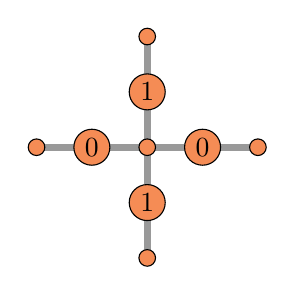
\begin{tikzpicture}[x=2em,y=2em,scale=1.0]
\draw[line width=2.5\pgflinewidth,pGray] (-2,0)--(2,0);
\draw[line width=2.5\pgflinewidth,pGray] (0,-2)--(0,2);
\node[circ] at (-1, 0) {$0$};
\node[circ] at ( 1, 0) {$0$};
\node[circ] at ( 0,-1) {$1$};
\node[circ] at ( 0, 1) {$1$};
\node[vert] at ( 0, 0) {};
\node[vert] at (-2, 0) {};
\node[vert] at ( 2, 0) {};
\node[vert] at ( 0,-2) {};
\node[vert] at ( 0, 2) {};
\end{tikzpicture}

\tikzsetnextfilename{6-vertex-model-4}
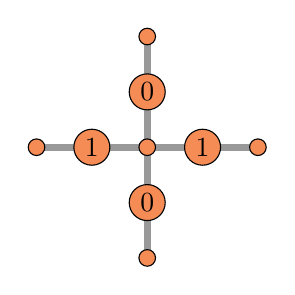
\begin{tikzpicture}[x=2em,y=2em,scale=1.0]
\draw[line width=2.5\pgflinewidth,pGray] (-2,0)--(2,0);
\draw[line width=2.5\pgflinewidth,pGray] (0,-2)--(0,2);
\node[circ] at (-1, 0) {$1$};
\node[circ] at ( 1, 0) {$1$};
\node[circ] at ( 0,-1) {$0$};
\node[circ] at ( 0, 1) {$0$};
\node[vert] at ( 0, 0) {};
\node[vert] at (-2, 0) {};
\node[vert] at ( 2, 0) {};
\node[vert] at ( 0,-2) {};
\node[vert] at ( 0, 2) {};
\end{tikzpicture}

\tikzsetnextfilename{6-vertex-model-5}
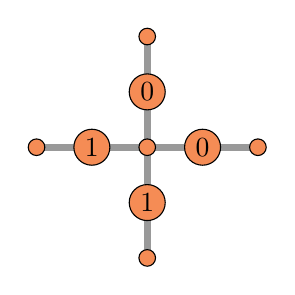
\begin{tikzpicture}[x=2em,y=2em,scale=1.0]
\draw[line width=2.5\pgflinewidth,pGray] (-2,0)--(2,0);
\draw[line width=2.5\pgflinewidth,pGray] (0,-2)--(0,2);
\node[circ] at (-1, 0) {$1$};
\node[circ] at ( 1, 0) {$0$};
\node[circ] at ( 0,-1) {$1$};
\node[circ] at ( 0, 1) {$0$};
\node[vert] at ( 0, 0) {};
\node[vert] at (-2, 0) {};
\node[vert] at ( 2, 0) {};
\node[vert] at ( 0,-2) {};
\node[vert] at ( 0, 2) {};
\end{tikzpicture}

\tikzsetnextfilename{6-vertex-model-6}
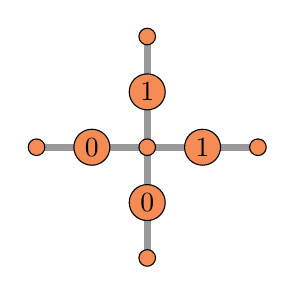
\begin{tikzpicture}[x=2em,y=2em,scale=1.0]
\draw[line width=2.5\pgflinewidth,pGray] (-2,0)--(2,0);
\draw[line width=2.5\pgflinewidth,pGray] (0,-2)--(0,2);
\node[circ] at (-1, 0) {$0$};
\node[circ] at ( 1, 0) {$1$};
\node[circ] at ( 0,-1) {$0$};
\node[circ] at ( 0, 1) {$1$};
\node[vert] at ( 0, 0) {};
\node[vert] at (-2, 0) {};
\node[vert] at ( 2, 0) {};
\node[vert] at ( 0,-2) {};
\node[vert] at ( 0, 2) {};
\end{tikzpicture}

\end{document}

